\documentclass{beamer}
\usepackage{graphicx}
\usepackage{tikz}
\usetikzlibrary{shapes,arrows}
\usepackage{tikz}
\usetheme{default}
%\usecolortheme{seahorse}

  \setbeamertemplate{footline}[page number]
\setbeamertemplate{navigation symbols}{}
\setbeamertemplate{frametitle}[default][center]
\setbeamerfont{frametitle}{shape=\scshape}

\usepackage{color}

\usepackage{media9}%
\newcommand{\includemovie}[3]{%
\includemedia[%
width=#1,height=#2,%
activate=pagevisible,%
deactivate=pageclose,%
addresource=#3,%
flashvars={%
src=#3 % same path as in addresource!
&autoPlay=true % default: false; if =true, automatically starts playback after activation (see option ?activation)?
&loop=true % if loop=true, media is played in a loop
&controlBarAutoHideTimeout=0 %  time span before auto-hide
}%
]{}{StrobeMediaPlayback.swf}}%


{\title{\textsc{Numerical Methods-Lecture VIII: Interpolation} \\ \  \\ \tiny (See Judd Chapter 6)}
\author{Trevor Gallen}
\date{}

\begin{document}

\begin{frame}
\titlepage
\end{frame}

\begin{frame}
\frametitle[alignment=center]{Warning}
\begin{itemize}
\item Over last few years I've noticed students don't use interpolation I teach here
\bigskip
\item Easier to use built-in Matlab
\bigskip
\item I'll run you through it because it is good to know the vulnerabilities and how we can avoid them
\bigskip
\item But I won't dwell on equations
\end{itemize}
\end{frame}

\begin{frame}
\frametitle[alignment=center]{Motivation}
\begin{itemize}
\item Most solutions are functions
\bigskip
\item Many functions are (potentially) high-dimensional
\bigskip
\item Want a way to simplify
\bigskip
\item A cloud of points and connecting the dots is one way
\bigskip
\item How should we connect the dots (and choose where they are?)
\end{itemize}
\end{frame}

\begin{frame}
\frametitle[alignment=center]{The most basic}
\begin{itemize}
\item The basics:
\bigskip
\begin{itemize}
\item Evenly-spaced grid, Connect the dots
\bigskip
\item Linearly or quadratically summarize the line
\end{itemize}
%\item Isn't this good enough, as number of points $\rightarrow \infty$?
\end{itemize}
\end{frame}

\begin{frame}
\frametitle[alignment=center]{Polynomial Basis}
\begin{itemize}
\item We can summarize functions with different bases
\bigskip
\item The most common is the polynomial basis:
\bigskip
 $$f(x) = \left[\begin{array}{ccccc}a_0 & a_1 & a_2 & \cdots & a_n\end{array}\right]\left[\begin{array}{cccc}1 \\ x \\ x^2 \\ \vdots \\ x^{n}\end{array}\right]$$
 \bigskip
\item This is really just the taylor polynomial:
\bigskip
$$f(x)=a_0+a_1x+a_2x^2+...+a_nx^n$$
\bigskip
\item But the polynomials are really colinear
\bigskip
\item This is pretty inefficient coding
\end{itemize}
\end{frame}

\begin{frame}
\frametitle[alignment=center]{Monomial Basis}
\begin{figure}
\centering
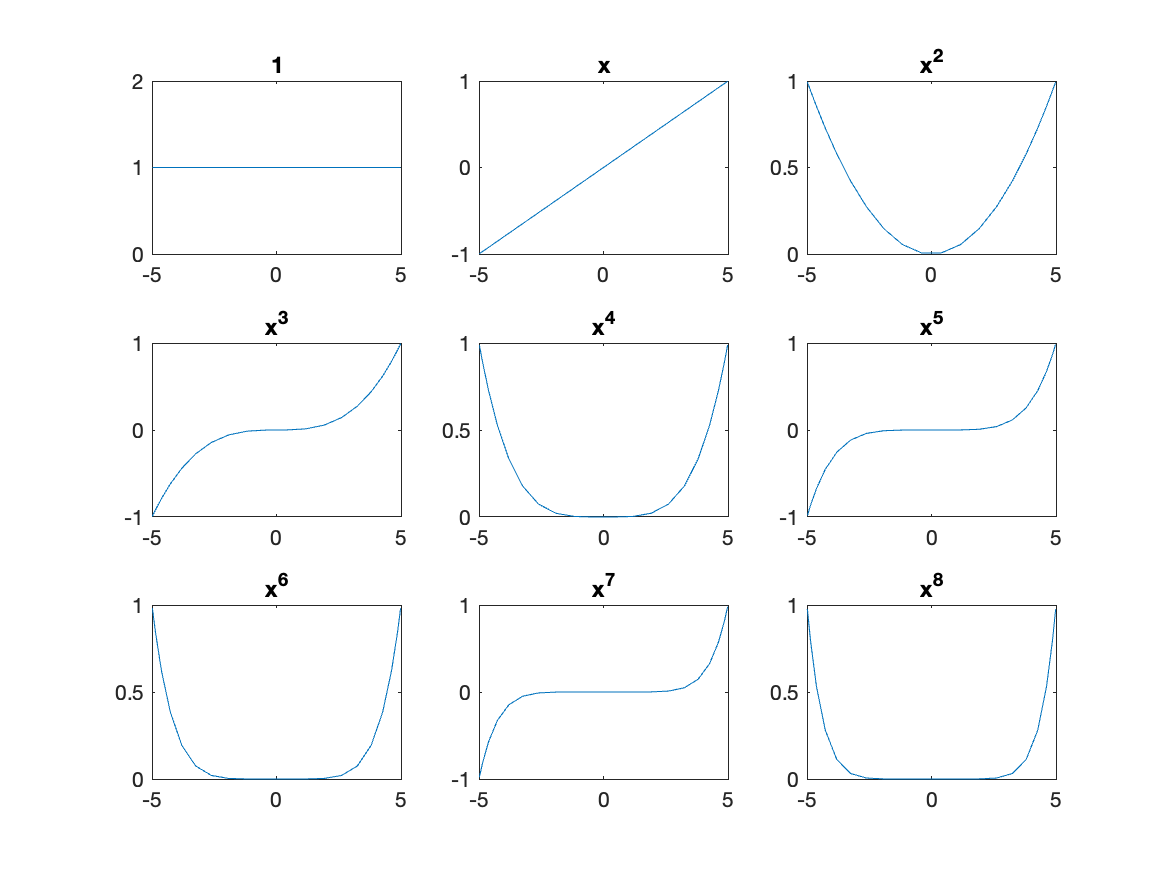
\includegraphics[scale=0.5]{Bases_Monomial.png}
\end{figure}
\end{frame}

\begin{frame}
\frametitle[alignment=center]{Example: ``Regression"}
\begin{itemize}
\item Have a cloud of $n$ points (data is $Y$), location in grid summarized by $X$
\bigskip
\item Regress cloud on polynomial basis of dimension $i$, $i<n$:
$$\hat{\beta}=(X'*X)^{-1}X'*Y$$
\item Then your interpolation is always just:
$$\hat{Y}=\hat{\beta}X$$
\item This is okay for a lot of problems
\end{itemize}
\end{frame}

\begin{frame}
\frametitle[alignment=center]{Example: ``Regression"}
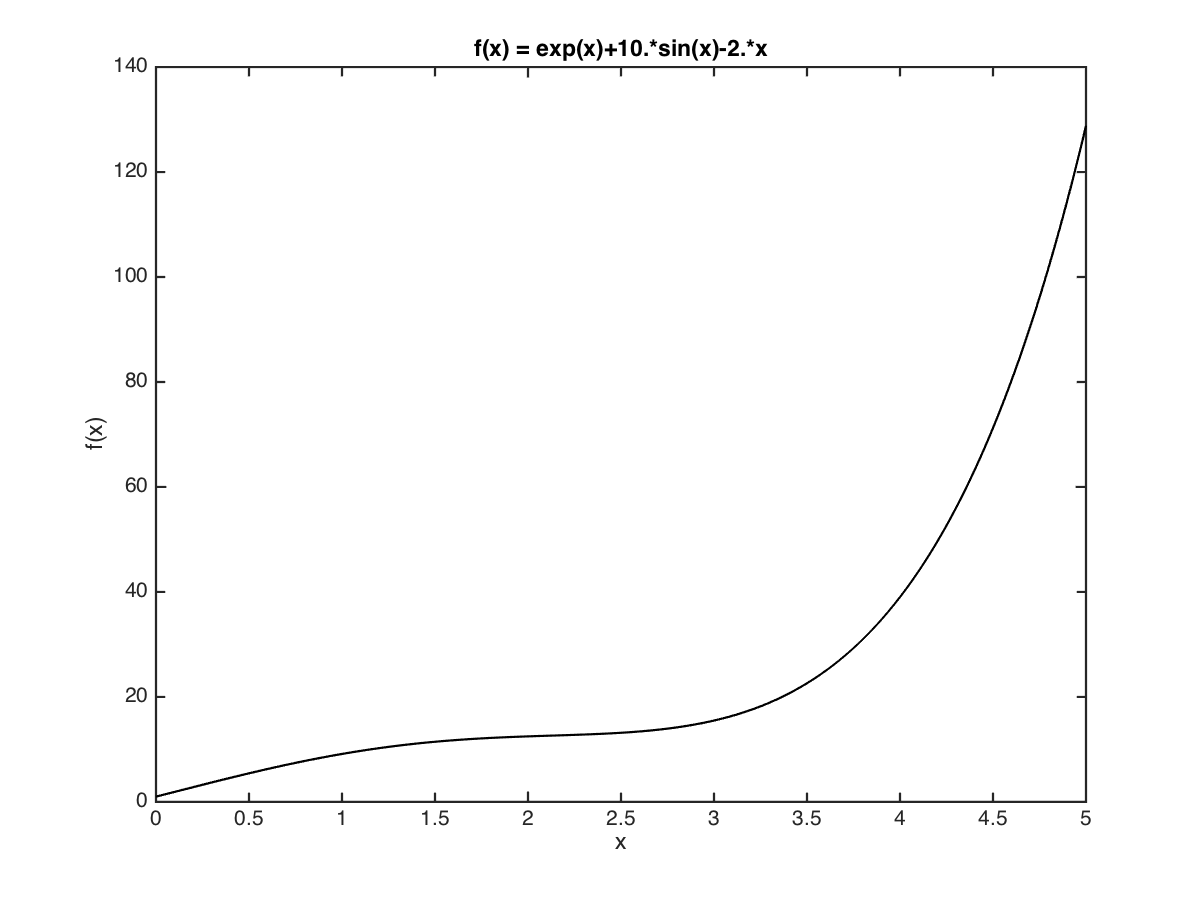
\includegraphics[scale=0.5]{Simple_m1.png}
\end{frame}


\foreach \x in {1,2,...,5}
{
\begin{frame}
\frametitle[alignment=center]{Example: ``Regression"}
\includegraphics[scale=0.5]{Simple_\x.png}
\end{frame}
}

\begin{frame}
\frametitle[alignment=center]{Runge's Phenomenon: $f(x)=\frac{1}{1+x.^2}$}
\begin{figure}
\centering
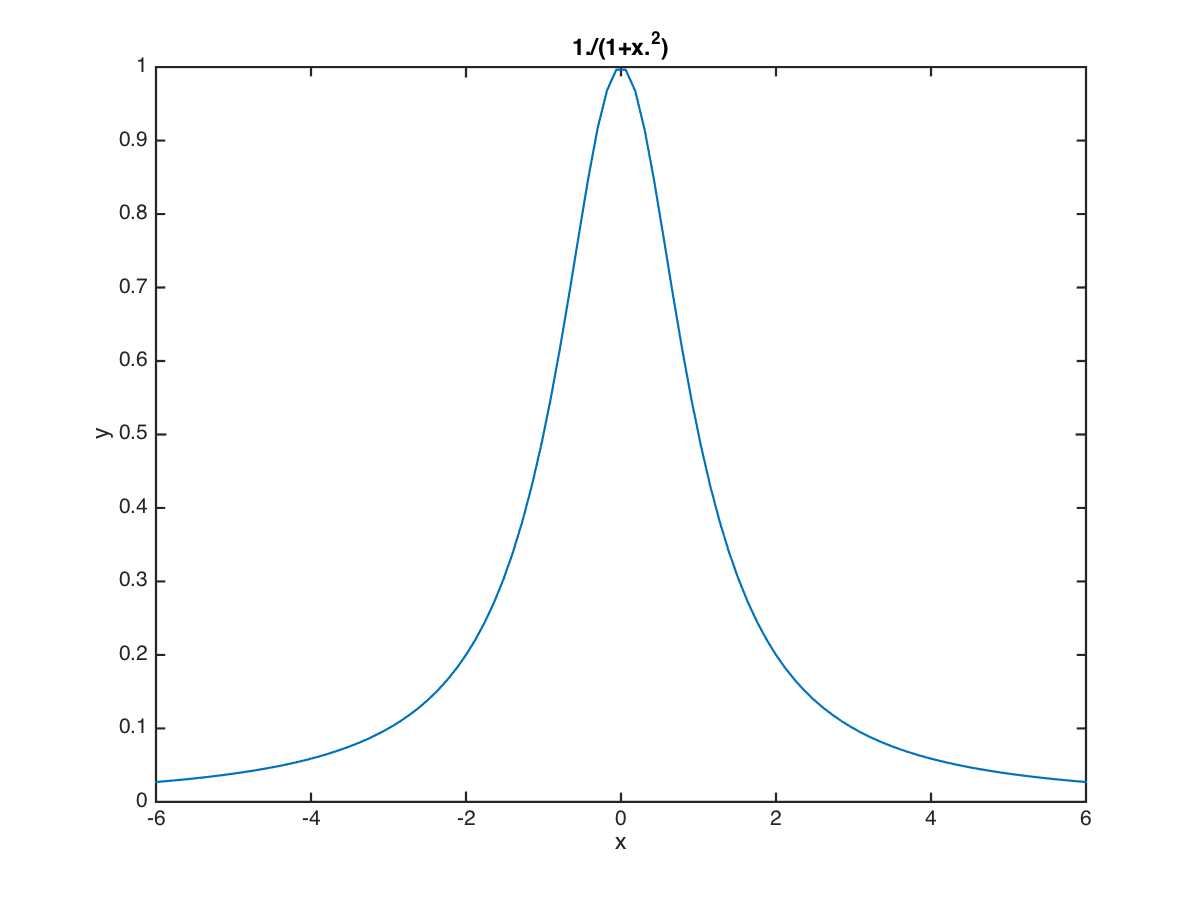
\includegraphics[scale=0.5]{Test_Function.png}
\end{figure}
\end{frame}

\foreach \x in {1,2,...,13}
{
\begin{frame}
\frametitle[alignment=center]{Approx: $f(x)=\frac{1}{1+x.^2}$: \x-deg. approx}
\begin{figure}
\centering
\includegraphics[scale=0.5]{Monom_1D_\x.png}
\end{figure}
\end{frame}
}

\foreach \x in {1,2,...,13}
{
\begin{frame}
\frametitle[alignment=center]{Errors: $f(x)=\frac{1}{1+x.^2}$: \x-deg. approx}
\begin{figure}
\centering
\includegraphics[scale=0.5]{Monom_1D_err_zoom\x.png}
\end{figure}
\end{frame}
}

\foreach \x in {1,2,...,13}
{
\begin{frame}
\frametitle[alignment=center]{Errors: $f(x)=\frac{1}{1+x.^2}$: \x-deg. approx}
\begin{figure}
\centering
\includegraphics[scale=0.5]{Monom_1D_err_\x.png}
\end{figure}
\end{frame}
}



\begin{frame}
\frametitle[alignment=center]{Chebychev Polynomials}
\begin{itemize}
\item Less violent and colinear polynomials are desirable
\item We also want something that avoids Runge's phenomenon if possible
\item We also want something that's pretty ``easy" to integrate 
\item It just so happens Chebychev polynomials are all of these things
\item Defined recursively:
$$T_0(x)=1$$
$$T_1(x)=x$$
$$T_{n}(x)=2xT_{n-1}(x)-T_{n-2}(x)$$
\item Defined over [-1,1]!  Needs transformation.
\end{itemize}
\end{frame}

\begin{frame}
\frametitle[alignment=center]{Chebychev Basis}
\begin{figure}
\centering
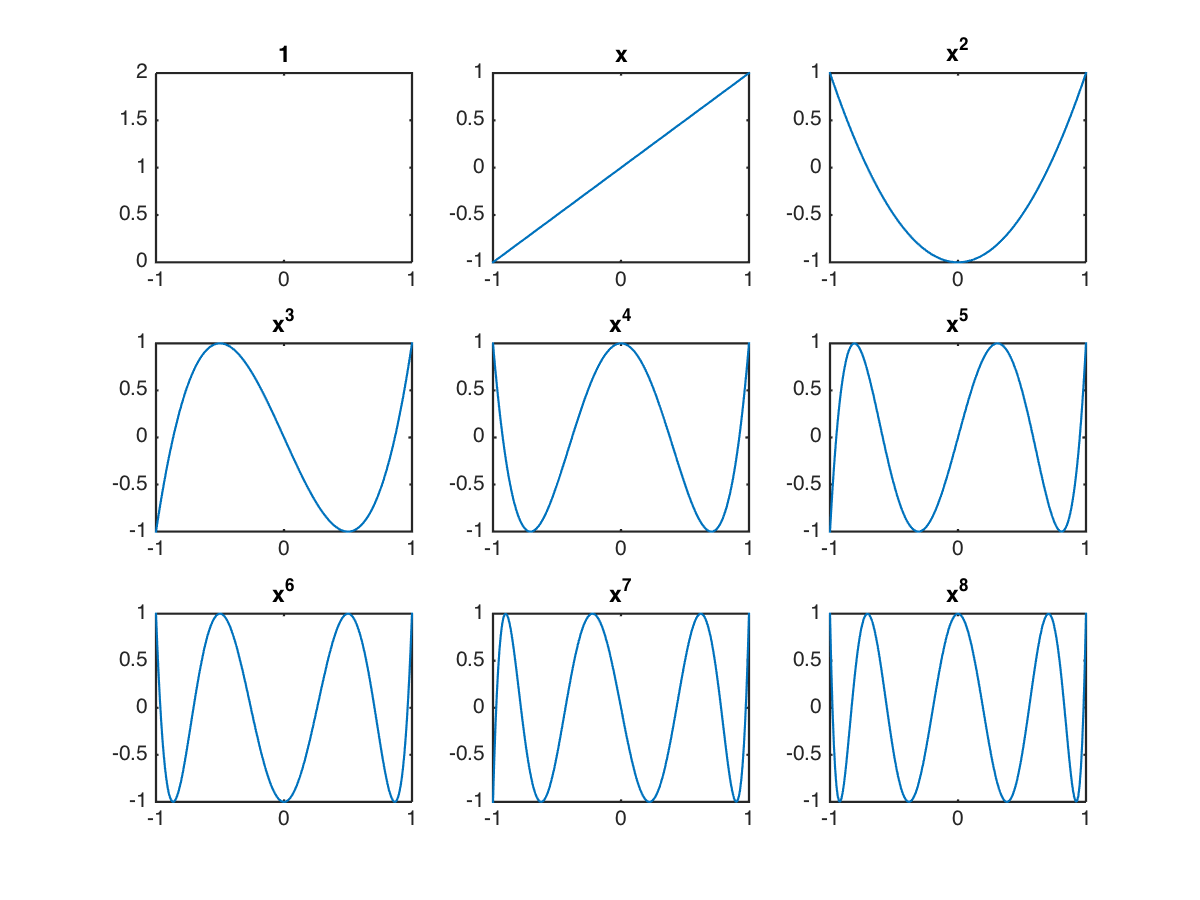
\includegraphics[scale=0.5]{Bases_Chebychev.png}
\end{figure}
\end{frame}

\begin{frame}
\frametitle[alignment=center]{Properties}
\begin{itemize}
\item Also can show that:
$$T_n(x)=cosh(n\cdot arccosh(x))$$
\item And that the roots $x_j^*$ $T_n$ are:
$$x_j=cos\left(\frac{2j-1}{2n}\pi\right)\ \ \ j=1,...,n$$
\item It just so happens that sampling at Chebychev nodes help minimize the maximum error and make sure it's monotonically decreasing as $n$ increases
\end{itemize}
\end{frame}

\begin{frame}
\frametitle[alignment=center]{Interpolation: 1-d}
\begin{itemize}
\item You have some function $f(x)$ that you want to interpolate over $[a,b]$.
\item Define a bridge between your range and the interpolating polynomial's range:
\item Define: $z=2(x-a)/(b-a)-1$, or $x=a+\frac{(b-a)(z+1)}{2}$
\item Then 
\begin{itemize}
\item $x=a\Rightarrow z=-1$
\item $x=b\Rightarrow z=1$
\item $x=(a+b)/2\Rightarrow z=0$.
\end{itemize}
\item Our goal will be, for interpolating polynomial $g(z)$ over $[-1,1]$ and $f(x)$ over $[a,b]$, that:
$$g(2(x-a)/(b-a)-1)=f(x)\ \ \ \forall x$$
\end{itemize}
\end{frame}

\begin{frame}
\frametitle[alignment=center]{Interpolation: 1-d}
\begin{enumerate}
\item Pick fcn. $f(x)$, degree $n$, bounds $a,b$ for interpolation.
\item Find Chebychev nodes for $f(x)$ in ``z" space. 
$$z_j=-cos\left(\frac{2j-1j}{2n}\pi\right)\ \ \ j=1,...,n$$
\item Convert nodes into ``x'' space:
$$x_j=a+\frac{(b-a)(z_j+1)}{2}$$
\item Calculate $y_j=f(x_j)$ at each $x_j$.  This is the value of $g(z_j)$ at each of the corresponding nodes.
\item Given $y_j$, calculate the Chebychev coefficients $c_j$ as:
$$c_j=\frac{2}{n+1}\sum_{k=0}^ny_jT_j(z_j)$$
\item Your approximation is given by:
$$\hat{f}(x)=\sum_{j}c_jT_j(x)\approx f(x)$$
\end{enumerate}
\end{frame}

\foreach \x in {2,...,13}
{
\begin{frame}
\frametitle[alignment=center]{Fit: $f(x)=\frac{1}{1+x.^2}$: \x-deg. approx}
\begin{figure}
\centering
\includegraphics[scale=0.5]{Cheby_1D_\x.png}
\end{figure}
\end{frame}
}

\foreach \x in {2,...,13}
{
\begin{frame}
\frametitle[alignment=center]{Errors: $f(x)=\frac{1}{1+x.^2}$: \x-deg. approx}
\begin{figure}
\centering
\includegraphics[scale=0.5]{Cheby_1D_err_\x.png}
\end{figure}
\end{frame}
}

\begin{frame}
\frametitle[alignment=center]{Interpolation: 2-d}
\begin{enumerate}
\item Pick fcn $f(x,y)$ deg. $n$, bounds a,b and c,d for interpolation.
\item Find Chebychev nodes for $f(x,y)$ in ``$z^{[1]}$" and ``$z^{[2]}$'' space. 
$$z^{[1]}_j=cos\left(\frac{2j-1j}{2n}\pi\right),\ \ \ \ \ \ \ z^{[2]}_j=cos\left(\frac{2j-1j}{2n}\pi\right),\ \ \ j=1,...,n$$
\item Convert nodes into ``x'' space:
$$x_j=a+\frac{(b-a)(z_j^{[1]}+1)}{2},\ \ \ y_j=c+\frac{(d-c)(z_j^{[2]}+1)}{2}$$
\item Calculate $\xi_{i,j}=f(x_i,y_j)$ for all points.
\item Given $y_j$, calculate the Chebychev coefficients $c_j$ as:
$$c_{i,j}=\frac{\sum_{k=1}^n\sum_{l=1}^n \xi_{i,j}T_i(z^{[1]}_k)T_j(z^{[2]}_l)}{\sum_{k=1}^n T_i(z^{[1]}_k)T_j(z^{[2]}_l)}$$
\item Approximation: 
$$\hat{f}(x,y)\approx \sum_{i=1}^n\sum_{j=1}^n c_{ij}T_i\left(2\frac{x-a}{b-a}-1\right)T_j\left(2\frac{y-c}{d-b}-1\right)$$
\end{enumerate}
\end{frame}


\foreach \x in {1,...,5}{
\begin{frame}
\frametitle[alignment=center]{Monom Fit: $f(x)=\frac{1}{1+x.^2}$: \x-deg. approx}
\begin{figure}
\centering
\includegraphics[scale=0.5]{Monom_2D_\x.png}
\end{figure}
\end{frame}
}

\foreach \x in {1,...,5}{
\begin{frame}
\frametitle[alignment=center]{Monom Errors: $f(x)=\frac{1}{1+x.^2}$: \x-deg. approx}
\begin{figure}
\centering
\includegraphics[scale=0.5]{Monom_2D_\x_err.png}
\end{figure}
\end{frame}
}



\foreach \x in {1,...,10}{
\begin{frame}
\frametitle[alignment=center]{Cheby Fit: $f(x)=\frac{1}{1+x.^2}$: \x-deg. approx}
\begin{figure}
\centering
\includegraphics[scale=0.5]{Cheby_2D_\x.png}
\end{figure}
\end{frame}
}

\foreach \x in {1,...,10}{
\begin{frame}
\frametitle[alignment=center]{Cheby Errors: $f(x)=\frac{1}{1+x.^2}$: \x-deg. approx}
\begin{figure}
\centering
\includegraphics[scale=0.5]{Cheby_2D_Err\x.png}
\end{figure}
\end{frame}
}

\begin{frame}
\frametitle[alignment=center]{Taste of some technical points}
\begin{itemize}
\item If we have some function $f(x)$ and some class of approximating functions, $\Omega$
\item We want to find the function $\omega(x)\in\Omega$ such that:
$$\omega=\underset{\omega\in\Omega}{\arg\min}||f-g||^2$$
\item Interpolating at Chebychev nodes allows us to obtain a lower bound for the error:
$$|f(x)-\hat{f}_{n-1}(x)|\leq \frac{1}{2^{n-1}n!}\underset{\xi\in[-1,1]}{\max}|f^{(n)}(\xi)|$$
\item For more see Judd Chapter 6: many ways to approximate functions.
\end{itemize}
\end{frame}

\begin{frame}
\frametitle[alignment=center]{Practical Note-I}
\begin{itemize}
\item As mentioned, I've found that this discussion of interpolation is not frequently used by students in research
\bigskip
\item Easier to use canned commands
\bigskip
\item In matlab, interpolation is relatively easy
\bigskip
\item Give it the basis for the function and the function, create an interpolating (and potentially extrapolating function)
\end{itemize}
\end{frame}

\begin{frame}
\frametitle[alignment=center]{Practical Note-II}
\begin{itemize}
\item General Matlab interpolation methods
\begin{itemize}
\item Linear - connect the dots with a line or plane
\item Nearest, next, previous - rarely used
\item Spline:  Fit points with local  polynomials of (typically) degree three
\item PChip:  Spline but doesn't overshoot (good for non-smooth functions)
\item Makima:  spline with orthogonal basis vectors
\end{itemize}
\end{itemize}
\end{frame}

\begin{frame}
\frametitle[alignment=center]{Practical Note-III}
\begin{itemize}
\item How does it work?
\bigskip
\item Let's say I want to define a value function in three dimensions:\\
\texttt{wvec = linspace(0,10,5)}\\
\texttt{mvec = [0,1]}\\
\texttt{cvec = [0,1,2,3,4]}\\
\texttt{[mgrid,wgrid,cgrid] = ndgrid(wvec,mvec,cvec)}\\
\texttt{V=rand(size(wgrid))}\\
\texttt{Vfxn = griddedInterpolant(wgrid,mgrid,cgrid,V)}\\
\texttt{Vfxn(2,1,2)}\\
\item Could also use:\\
 \texttt{scatteredInterpolant(xvec1,xvec2,xvec3,yvec)}\\
 for scattered/non-gridded data.
\end{itemize}
\end{frame}

\begin{frame}
\frametitle[alignment=center]{Practical Note-IV}
\begin{itemize}
\item Making grids in Matlab
\bigskip
\item Two commands: ndgrid (interpolation) and meshgrid (ease of graphing)
\item $[a,b]=meshgrid([1:2],[3:4])$ gives:
$$a=\left[\begin{array}{cc}1 & 2 \\ 1 & 2\end{array}\right]\ \ b=\left[\begin{array}{cc}3 & 3 \\ 4 & 4\end{array}\right]$$
\item $[a,b]=ndgrid([1:2],[3:4])$ gives:
$$a=\left[\begin{array}{cc}1 & 1 \\ 2 & 2\end{array}\right]\ \ b=\left[\begin{array}{cc}3 & 4 \\ 3 & 4\end{array}\right]$$
\item Matlab expects things to be in ndgrid format for interpolation (while surf uses meshgrid)
\bigskip
\item Can always transpose, but if things aren't working, check if this is a problem.  Useful to have different \#'s of indicies so interp crashes if things are in wrong order
\end{itemize}
\end{frame}



\end{document}